\chapter{Lab 7 - Capacitor Applications}

%%%%%%%%%%%%%%%%%%%%%%%%%%%%%%%%%%%%%%%%%%%%%%%%%%%%%%%%%%%%%%%%%%%%%%%%%%%%%%%%%%%%%%%%%%%%%%%%%%%%%%%
\section{Objective}
%%%%%%%%%%%%%%%%%%%%%%%%%%%%%%%%%%%%%%%%%%%%%%%%%%%%%%%%%%%%%%%%%%%%%%%%%%%%%%%%%%%%%%%%%%%%%%%%%%%%%%%

The objective of this lab is to introduce another fundamental circuit element, the capacitor, and their applications within certain circuits. Specifiably for this lab, the focus is on a capacitor used in conjunction with a 555 timer. 

%%%%%%%%%%%%%%%%%%%%%%%%%%%%%%%%%%%%%%%%%%%%%%%%%%%%%%%%%%%%%%%%%%%%%%%%%%%%%%%%%%%%%%%%%%%%%%%%%%%%%%%
\section{Materials}
%%%%%%%%%%%%%%%%%%%%%%%%%%%%%%%%%%%%%%%%%%%%%%%%%%%%%%%%%%%%%%%%%%%%%%%%%%%%%%%%%%%%%%%%%%%%%%%%%%%%%%%

\begin{itemize}
	\item Laptop with LTSpice
	\item Analog Discovery
	\item Breadboard
	\item Wiring kit
	\item Lab parts kit 
\end{itemize}

%%%%%%%%%%%%%%%%%%%%%%%%%%%%%%%%%%%%%%%%%%%%%%%%%%%%%%%%%%%%%%%%%%%%%%%%%%%%%%%%%%%%%%%%%%%%%%%%%%%%%%%
\section{Introduction}
%%%%%%%%%%%%%%%%%%%%%%%%%%%%%%%%%%%%%%%%%%%%%%%%%%%%%%%%%%%%%%%%%%%%%%%%%%%%%%%%%%%%%%%%%%%%%%%%%%%%%%%

There are a variety of applications of capacitors which could fill an entire class. The focus for this lab will be the use of a capacitor and its associated RC time constant in conjunction with a 555 timer. 

%%%%%%%%%%%%%%%%%%%%%%%%%%%%%%%%%%%%%%%%%%%%%%%%%%%%%%%%%%%%%%%%%%%%%%%%%%%%%%%%%%%%%%%%%%%%%%%%%%%%%%%
\subsection{Time Domain Response}
%%%%%%%%%%%%%%%%%%%%%%%%%%%%%%%%%%%%%%%%%%%%%%%%%%%%%%%%%%%%%%%%%%%%%%%%%%%%%%%%%%%%%%%%%%%%%%%%%%%%%%%

While the operation of a capacitor can be analyzed in both the time and frequency domains, the focus here is on the time domain. 

\begin{figure}
	\centering
		\includegraphics[width=1\textwidth]{Lab5cap.pdf}
	\caption{A simple RC circuit (a) and the associated input and output (b). Note that the input is the node after the switch in (a).} \label{fig:capoutput}
\end{figure}

A simple RC circuit with a switch as shown in \hyperref[fig:capoutput]{Figure \ref*{fig:capoutput}} will charge and discharge as the 1 V source is connected and disconnected. Charging to the source voltage takes the form of 

\begin{equation}
	\centering
	V_{out} = 1 - V_{in}e^{-t/\tau}
\end{equation}

\noindent where $\tau = RC$ and discharging takes the form

\begin{equation}
	\centering
	V_{out} =  V_{in}e^{-t/\tau}
\end{equation}

\noindent While the result is novel and opens up a lot of possibilities, there isn't a clear path to the actual application of the capacitor. Sure, it can be used in the previously mentioned simple RC circuit, but there isn't a clear use. Enter the 555 timer, an early chip that because incredibly popular due to the ability to generate various timing signals using external components to set an RC time constant. 

%%%%%%%%%%%%%%%%%%%%%%%%%%%%%%%%%%%%%%%%%%%%%%%%%%%%%%%%%%%%%%%%%%%%%%%%%%%%%%%%%%%%%%%%%%%%%%%%%%%%%%%
\subsection{555 Timer}
%%%%%%%%%%%%%%%%%%%%%%%%%%%%%%%%%%%%%%%%%%%%%%%%%%%%%%%%%%%%%%%%%%%%%%%%%%%%%%%%%%%%%%%%%%%%%%%%%%%%%%%

A 555 timer can operate in two modes, mono-stable  and a-stable. Mono-stable operating is when the circuit will only output once when triggered and will wait for future triggers to output again. A-stable operating requires no input and will internally trigger to perpetually produce output. 

For clarification, there is a distinction between the pulse duration, the time a signal is high (highest positive voltage, usually the positive voltage rail) and the period. \hyperref[fig:7durvsper]{Figure \ref*{fig:7durvsper}} shows the difference between the pulse duration and period for a square wave. The pulse duration is time the square wave is at its maximum value, 1 V in this case, for a total of 0.25 ms. While the period is the time it takes for the signal to repeat, 0.5 ms. 

\begin{figure}
	\centering
		\includegraphics[width=0.5\textwidth]{lab7durvsper.pdf}
	\caption{A plot of a square wave with the pulse duration and period labeled.} \label{fig:7durvsper}
\end{figure}

\newpage

%%%%%%%%%%%%%%%%%%%%%%%%%%%%%%%%%%%%%%%%%%%%%%%%%%%%%%%%%%%%%%%%%%%%%%%%%%%%%%%%%%%%%%%%%%%%%%%%%%%%%%%
\subsubsection{Mono-Stable Configuration}
%%%%%%%%%%%%%%%%%%%%%%%%%%%%%%%%%%%%%%%%%%%%%%%%%%%%%%%%%%%%%%%%%%%%%%%%%%%%%%%%%%%%%%%%%%%%%%%%%%%%%%%

The mono-stable configuration, \hyperref[fig:monostable]{Figure \ref*{fig:monostable}}, requires an input and only triggers when that input passes below a specific threshold (active low). Once the input falls below the threshold voltage, the output goes to 5 V for $t=  1.1 R_A C_L$ and the capacitor starts to charge. Once the capacitor voltage reaches a threshold, the output and the capacitor voltage both go to zero and the circuit waits for the input voltage to go zero again. 

\begin{figure}
	\centering
		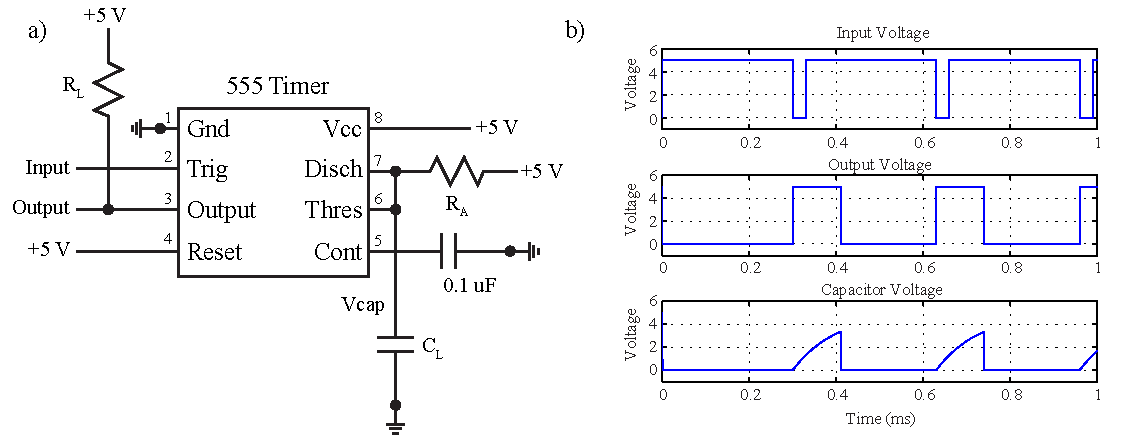
\includegraphics[width=0.9\textwidth]{Lab5monostable.pdf}
	\caption{The circuit for mono-stable operation (a) and the output voltages (b). Vcc is 5 V, $R_L = 1\mathrm{k}\; \Omega$, $C_L = 0.01\mu \mathrm{F}$, and $R_A = 10\mathrm{k}\;\Omega$. Note that wires that cross are only connected if there is a dot at the junction.} \label{fig:monostable}
\end{figure}



%%%%%%%%%%%%%%%%%%%%%%%%%%%%%%%%%%%%%%%%%%%%%%%%%%%%%%%%%%%%%%%%%%%%%%%%%%%%%%%%%%%%%%%%%%%%%%%%%%%%%%%
\subsubsection{A-Stable Configuration}
%%%%%%%%%%%%%%%%%%%%%%%%%%%%%%%%%%%%%%%%%%%%%%%%%%%%%%%%%%%%%%%%%%%%%%%%%%%%%%%%%%%%%%%%%%%%%%%%%%%%%%%

The a-stable configuration, \hyperref[fig:astable]{Figure \ref*{fig:astable}}, does not require an input  and utilizes the charging and discharging of the capacitor to trigger the input. With the addition of a second resistor, $R_B$, the capacitor will charge through resistors $R_A$ and $R_B$ but the capacitor will only discharge through $R_B$, leading to two different time constants. 

As the capacitor discharges, the output is zero until the capacitor voltage reaches the lower threshold voltages and then the output goes to 5 V until the capacitor voltage reaches the upper threshold and the process repeats. 

\begin{figure}[h]
	\centering
		\includegraphics[width=0.9\textwidth]{Lab5astable.pdf}
	\caption{The circuit for a-stable operation (a) and the output voltages (b). Vcc is 5 V, $R_L = 1\mathrm{k}\; \Omega$, $C_L = 0.01\mu \mathrm{F}$, $R_A = 10k\;\Omega$, and $R_B = 10\mathrm{k}\;\Omega$. Note that wires that cross are only connected if there is a dot at the junction.} \label{fig:astable}
\end{figure}

The time that the output is high is set by the two resistors and capacitor:

\begin{equation}
	\centering
	t_H = 0.693(R_A + R_B)C_L
\end{equation}

\noindent While the time the output is low is only set by $R_B$ and the capacitor:

\begin{equation}
	\centering
	t_L = 0.693(R_B)C_L
\end{equation}

%%%%%%%%%%%%%%%%%%%%%%%%%%%%%%%%%%%%%%%%%%%%%%%%%%%%%%%%%%%%%%%%%%%%%%%%%%%%%%%%%%%%%%%%%%%%%%%%%%%%%%%
\section{Big Picture}
%%%%%%%%%%%%%%%%%%%%%%%%%%%%%%%%%%%%%%%%%%%%%%%%%%%%%%%%%%%%%%%%%%%%%%%%%%%%%%%%%%%%%%%%%%%%%%%%%%%%%%%

While capacitors are used in the finale project, they're used for filtering purposes as opposed to use in the time domain with the 555 timer. 

%%%%%%%%%%%%%%%%%%%%%%%%%%%%%%%%%%%%%%%%%%%%%%%%%%%%%%%%%%%%%%%%%%%%%%%%%%%%%%%%%%%%%%%%%%%%%%%%%%%%%%%
\section{Pre-Lab Requirements}
%%%%%%%%%%%%%%%%%%%%%%%%%%%%%%%%%%%%%%%%%%%%%%%%%%%%%%%%%%%%%%%%%%%%%%%%%%%%%%%%%%%%%%%%%%%%%%%%%%%%%%%

Complete the following before coming to lab. 

%%%%%%%%%%%%%%%%%%%%%%%%%%%%%%%%%%%%%%%%%%%%%%%%%%%%%%%%%%%%%%%%%%%%%%%%%%%%%%%%%%%%%%%%%%%%%%%%%%%%%%%
\subsection{LTspice Simulations} \label{ssec:sims}
%%%%%%%%%%%%%%%%%%%%%%%%%%%%%%%%%%%%%%%%%%%%%%%%%%%%%%%%%%%%%%%%%%%%%%%%%%%%%%%%%%%%%%%%%%%%%%%%%%%%%%%

Using LTspice, complete the following. Use 5 V for Vcc, $R_L = 1\mathrm{k}\;\Omega$, and the NE555 model for the 555 timer found in the Misc component section. 

\begin{enumerate}
	\item Read the NE555 datasheet, \url{http://www.ti.com/product/NE555/datasheet}. Please note that a mono-stable allows for the pulse width to change as resistor and capacitor values are varied, while an a-stable configuration allows for the period the be varied as resistor and capacitor values are varied.
	\item Using the mono-stable configuration, determine the output when $R_A = 15\mathrm{k}\;\Omega$ and $C_L = 0.01 \mu \mathrm{F}$. Set the input to a pulse source with the following settings: 0 5 0 1n 1n 0.2m 0.25m 5 and run a transient simulation with a stop time of 1m (.tran 1m). Table the output voltage pulse duration, then save an image of the circuit and a plot of the input and output voltage for submission to Canvas. \label{itm:7ssec1itm1}
	\item Using the mono-stable configuration, choose $R_A$ and $C_L$ so that the output pulse duration is  approximtely 200 $\mu$s ($f\approx 5$ kHz) for a 100 kHz input; the solution should be withing 4 $\mu$s, 200 $\mu$s +/- 4 $\mu$s (5 kHz +/- 100 Hz). Use only the parts in your lab kit. Set the input to a pulse source with the following settings: 0 5 0 1n 1n 8u 10u 50 and run a transient simulation with a stop time of 0.5m (.tran 0.5m). Table the output voltage pulse duration, then save an image of the circuit and a plot of the input and output voltage for submission to Canvas. \label{itm:7ssec1itm2}
	\item Using the a-stable configuration, determine the output when $R_A = 10\mathrm{k}\;\Omega$, $R_B = 10\mathrm{k}\;\Omega$, and $C_L = 0.01 \mu \mathrm{F}$. Run a transient simulation with a stop time of 1m (.tran 1m). Table the output voltage period, then save an image of the circuit and a plot of the output voltage for submission to Canvas. \label{itm:7ssec1itm3}
	\item Using the a-stable configuration, choose $R_A$, $R_B$, and $C_L$ so that the frequency of the output signal is 10 kHz, there is an exact solution. Use only the parts in your lab kit. Run a transient simulation with a stop time of 0.5m (.tran 0.5m). Table the output voltage period, then save an image of the circuit and a plot of the output voltage for submission to Canvas. \label{itm:7ssec1itm4}
\end{enumerate}

%%%%%%%%%%%%%%%%%%%%%%%%%%%%%%%%%%%%%%%%%%%%%%%%%%%%%%%%%%%%%%%%%%%%%%%%%%%%%%%%%%%%%%%%%%%%%%%%%%%%%%%
\subsection{Breadboard Implementation} \label{ssec:breadboard}
%%%%%%%%%%%%%%%%%%%%%%%%%%%%%%%%%%%%%%%%%%%%%%%%%%%%%%%%%%%%%%%%%%%%%%%%%%%%%%%%%%%%%%%%%%%%%%%%%%%%%%%

\begin{enumerate}
	\item Build a mono-stable configuration  from \hyperref[itm:7ssec1itm1]{Section \ref*{ssec:sims} Item \ref*{itm:7ssec1itm1}}. Set Vcc to 5 V supply and use a 5 kHz square wave as the input with a 2.5 V amplitude and a 2.5 V offset. You can determine the capacitor values by their quantity or the labels: 102J - 0.001 $\mu$F, 103J - 0.01 $\mu$F, 333J - 0.033 $\mu$F, 473J - 0.047 $\mu$ F, 104J - 0.1 $\mu$ F, and 105K - 1 $\mu$F.
	\item Display the output voltage and the capacitor voltage on the o-scope to demonstrate the circuit to your lab instructor at the start of lab. In this case it helps to ground the negative terminals for the o-scope probes. 
\end{enumerate}

%%%%%%%%%%%%%%%%%%%%%%%%%%%%%%%%%%%%%%%%%%%%%%%%%%%%%%%%%%%%%%%%%%%%%%%%%%%%%%%%%%%%%%%%%%%%%%%%%%%%%%%
\section{In-Lab Requirements}
%%%%%%%%%%%%%%%%%%%%%%%%%%%%%%%%%%%%%%%%%%%%%%%%%%%%%%%%%%%%%%%%%%%%%%%%%%%%%%%%%%%%%%%%%%%%%%%%%%%%%%%

The following must be completed at the start of lab. 

\begin{enumerate}
	\item \hyperref[ssec:sims]{Subsection \ref*{ssec:sims}}
		\begin{enumerate} 
			\item \hyperref[itm:7ssec1itm1]{Item \ref*{itm:7ssec1itm1}}: An image of the circuit and a plot of the input and output voltage.
			\item \hyperref[itm:7ssec1itm2]{Item \ref*{itm:7ssec1itm2}}: An image of the circuit and a plot of the input and output voltage.
			\item \hyperref[itm:7ssec1itm3]{Item \ref*{itm:7ssec1itm3}}: An image of the circuit and a plot of the output voltage.
			\item \hyperref[itm:7ssec1itm4]{Item \ref*{itm:7ssec1itm4}}: An image of the circuit and a plot of the output voltage.
			\item Table of both theoretical pulse durations and periods. 
		\end{enumerate}
		\begin{enumerate}
			\item \hyperref[ssec:breadboard]{Section \ref*{ssec:breadboard}}: Mono-stable configuration implemented and working on a breadboard. 
		\end{enumerate}

\end{enumerate}

%%%%%%%%%%%%%%%%%%%%%%%%%%%%%%%%%%%%%%%%%%%%%%%%%%%%%%%%%%%%%%%%%%%%%%%%%%%%%%%%%%%%%%%%%%%%%%%%%%%%%%%
\subsection{Construction}
%%%%%%%%%%%%%%%%%%%%%%%%%%%%%%%%%%%%%%%%%%%%%%%%%%%%%%%%%%%%%%%%%%%%%%%%%%%%%%%%%%%%%%%%%%%%%%%%%%%%%%%

For all four cases, determine the experimental pulse durations/periods for the output voltage and table the resulting values. 

\begin{enumerate}
	\item Save an image of the output voltage and capacitor voltage on the o-scope for the circuit from \hyperref[ssec:breadboard]{Subsection \ref*{ssec:breadboard}}.
	\item Construct the circuit from \hyperref[itm:7ssec1itm2]{Section \ref*{ssec:sims} Item \ref*{itm:7ssec1itm2}} on a breadboard and save an image of the output voltage and capacitor voltage on the o-scope.
	\item Construct the circuit from \hyperref[itm:7ssec1itm3]{Section \ref*{ssec:sims} Item \ref*{itm:7ssec1itm3}} on a breadboard and save an image of the output voltage and capacitor voltage on the o-scope.
	\item Construct the circuit from \hyperref[itm:7ssec1itm4]{Section \ref*{ssec:sims} Item \ref*{itm:7ssec1itm4}} on a breadboard and save an image of the output voltage and capacitor voltage on the o-scope.
\end{enumerate}

%%%%%%%%%%%%%%%%%%%%%%%%%%%%%%%%%%%%%%%%%%%%%%%%%%%%%%%%%%%%%%%%%%%%%%%%%%%%%%%%%%%%%%%%%%%%%%%%%%%%%%%
\section{Write Up}
%%%%%%%%%%%%%%%%%%%%%%%%%%%%%%%%%%%%%%%%%%%%%%%%%%%%%%%%%%%%%%%%%%%%%%%%%%%%%%%%%%%%%%%%%%%%%%%%%%%%%%%

Include the following in the write up.

\begin{enumerate}
	\item All four plots from the in-lab section detailing the output voltage and capacitor voltage. 
	\item Tabled experimental pulse durations/periods for the output voltages and percent error when compared to the theoretical values in the pre-lab. Pre-lab values and pre-lab plots are not required. 
\end{enumerate}

Discuss the differences between the theoretical outputs from LTspice and the experimental outputs when implementing the circuits on a breadboard. Why would they be different and do the scope probes adversely affect the results? 


